\chapter{Introduction}
\label{chap:introduction}
%In this chapter we will give a short introduction to the project, why we have chosen to work in this area and where the focus in the rest of this report lies. \\

%This student report is written as part of a learning project. Therefore we must comply with the study regulation.
%The study regulation states that the main focus of this semester's project is to gain knowledge of, and develop: Internet applications, -agents, or -services.
%The goal is thus to create an Internet application that provides a service with focus on agent technologies, scalability, and data intensity. \\

When a crime occurs documentation is often needed in order to convict the person(s) responsible and to receive repairs from an insurance company for the damages suffered.
Documentation can be eye witnesses, forensic evidence, or video surveillance.
Documentation in the form of eye witnesses or forensic evidence are unreliable sources, as it is not possible to guarantee it will be available.
Video surveillance is however always obtainable, but it is far from a perfect solution in its current form.\fixme{Statement - source}

\section{Video Surveillance}\label{sec:video_surveillance}
Video surveillance is widely used to obtain documentation or evidence of a crime, or as a preventive tool.
As an example there is one camera for every 32 people in the United Kingdom \citep{london_camera_surveillance}.
This number includes both cameras installed by the government to surveil London, but also cameras installed by businesses to secure their property.
The high number of cameras is partially attributed to the high need for surveillance to prevent e.g. terrorist attacks, but additionally due to the technical difficulties of video surveillance. \\

A typical video surveillance solution consists of cameras connected via cables to a control station.
Video cameras are mounted on a fixed location, and can therefore only surveil an area limited by their field of view, see Figure~\ref{fig:camera_properties}, and the environment in which it is placed.\\

\begin{figure}[htb]
    \centering
    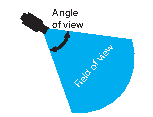
\includegraphics[scale=1.8]{gfx/camera_properties.pdf}
    \caption{A camera's field of view.}
    \label{fig:camera_properties}
\end{figure}

\fixme{Billedet skal opdateres så den lange streg fjernes}

An environment can contain physical objects which limits the camera's field of view further, see Figure~\ref{fig:refular_camera_setup}.
In small environments a sufficient degree of surveillance can be achieved without too much difficulty or cost (based on the interview described in Appendix~\ref{appendix:lytzen_it}).
Properly surveilling large areas is however problematic and can be expensive in regard to required hardware and installation costs such as digging down cables i.e.:

We have issues surveilling large areas, e.g. mink farms, with traditional solutions such as surveillance cameras.
The issues with a traditional solution for mink farms are that the establishment costs are very high due to e.g. digging.
% Vi har problemer med at overvåge store områder, som fx minkfarme, ved brug af en traditionel løsning i form af overvågningskameraer. Problemerne omkring en traditionel løsning til en minkfarm er at etableringsomkostninger er meget høje bl.a. på grund af gravearbejde.

%The need for video surveillance is based on the need for documentation of crimes, which is required in case of damage loses from an insurance perspective.
%Should a break-in occur a definitive proof of such must often be presented in order for insurances to cover potential losses.

A camera's field of view is not a hard limit for what it can record, however only what is recorded within the field of view is of high enough quality to be used as documentation.
%Video cameras have a limited field of view, both in terms of vision and range, and only within this field of view is the quality high enough be usable as documentation.
This limitation can make it difficult and resource intensive to surveil large areas.
The resource intensitivity stems from the amount of hardware required to surveil, referring both to cameras and cables needed to connect the surveillance system.
The difficulty in surveilling the areas comes from the nature of an outdoor environment.
In terms of surveillance an indoor environment can be seen as static, as there is a limited amount of entrances and the interior of the buildings in terms of walls and doors remain the same.
In an outdoor environment the weather has to be taken into account.
The weather can be foggy or rainy and the sun can blind a camera if it is improperly placed.
These conditions make video surveillance of outdoor areas difficult.
Both indoors and outdoors have some challenges that need to be faced, such as physical objects being moved around creating blind spots, etc.


\section{Current solutions}
This section will discuss some of the current solutions used for video surveillance, such as: regular camera, photo sensor, and dome camera.
The strengths and weaknesses of each solution will be covered.
The figures referenced in this section show the same area with a different surveillance setup to make them comparable. \\

In a regular camera solution, mounted cameras are used.
These cameras surveil a limited area, and in order to cover a larger area, multiple cameras are needed.
Multiple areas can be surveilled simultaneously with multiple cameras.
A limitation with a regular camera setup is that the cameras are stationary.
This means a cameras field of view can be limited by physical objects.
As an example in Figure~\ref{fig:refular_camera_setup} it can be seen how an object placed in a cameras field of view can create a blind spot in an area normally covered by a camera. \\

\begin{figure}[htb]
    \centering
    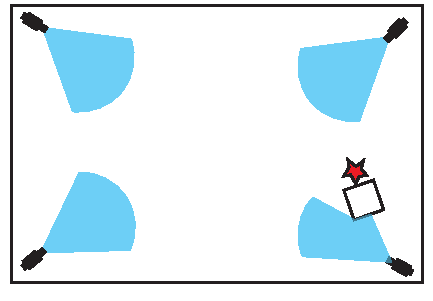
\includegraphics[width=\textwidth]{gfx/regular_camera_setup.pdf}
    \caption{Example of a Regular Camera Setup}
    \label{fig:refular_camera_setup}
\end{figure}

The red star in Figure ~\ref{fig:refular_camera_setup} represents a critical object, that needs to be observed. \\

In a photo sensor solution the perimeter of the surveilled area is covered by both cameras and photo sensors.
The purpose of the setup is to detect if anything enters the area, and then activate the cameras to capture it on video, as seen in Figure~\ref{fig:photo_sensor}.
A photo sensor solution can be used in combination with a regular camera solution, to surveil both the interior and the perimeter of an area.
The advantage of a photo sensor setup is that the cameras surveilling the perimeter are only activated if the sensors are triggered, ensuring video footage is only recorded when it is needed.
The disadvantage is that the cameras are still stationary, meaning the a large amount of cameras are required to surveil a large area. \\

\begin{figure}[htb]
    \centering
    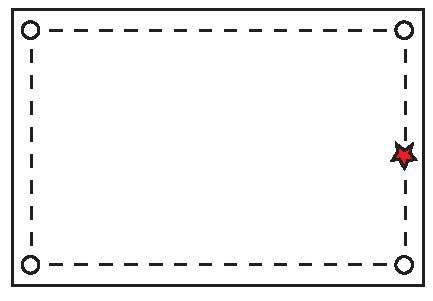
\includegraphics[width=\textwidth]{gfx/light_sensor.pdf}
    \caption{Example of a Photo Sensor Setup}
    \label{fig:photo_sensor}
\end{figure}

The next solution centers around having a dome camera with a long field of view in the center.
The perimeter is then divided into zones, by fx. light sensors.
When a zone have detected an entry, the dome camera is rotated towards that zone to observe the area.
Compared to the two previous solution, the dome camera solution is limited to only observe a specific subarea at a time, as seen in Figure~\ref{fig:drone_sensor}. \\

\begin{figure}[htb]
    \centering
    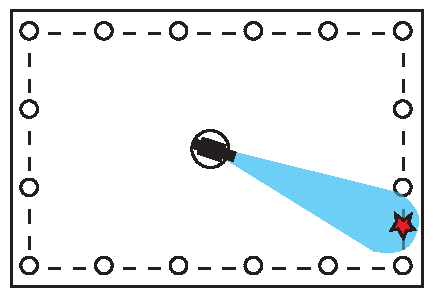
\includegraphics[width=\textwidth]{gfx/drome_sensor.pdf}
    \caption{Example of a Dome Setup}
    \label{fig:drone_sensor}
\end{figure}

\section{Drone Technology}
\section{Web for Surveillance}
With the development and standardization of network technologies, video surveillance is becoming digitized.
The digitization of video surveillance is important as it e.g. makes it faster to examine a video recording, and video cameras can be programmed to trigger alarms when they detect movement.
Video recordings are examined faster as it is easy to skip through digital data compared to the analog data which would be stored on e.g. a VHS cassette.
The programming of video cameras is possible due to the data being digital. 
It is possible to apply algorithms to examine the digital data, which could e.g. identify license plates on cars.
The digitization allows for the use of the Internet.
The Internet makes it possible to interconnect surveillance solution, that enables features such as backup or long distance observing.
\section{Problem Statement}
\label{sec:problem_definition}
Video surveillance in its current form is stationary, meaning cameras cannot move.
As a consequence of this, a large amount of hardware is required to properly surveil an area.
This is problematic when a large area has to be surveilled, because the cost of hardware is high and the larger the area the more hardware is to be used.
Drone technology offers a possible solution to this problem by making video surveillance dynamic through movable cameras.
This possible solution yields the following preliminary problem statement:\\

%http://guide-images.ifixit.net/igi/cI6EGVSLLjjDFATI.medium
\begin{figure}[htb]
    \centering
    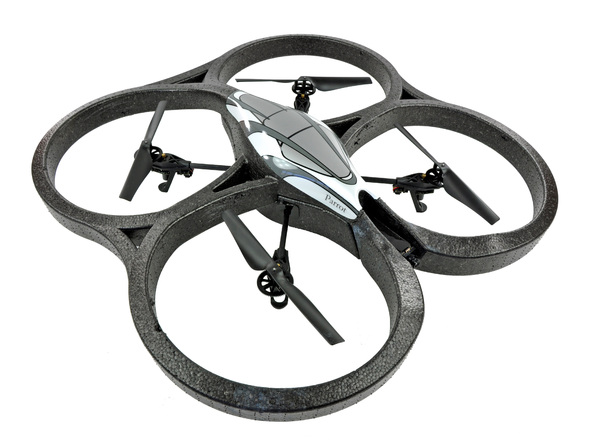
\includegraphics[width=\textwidth]{gfx/drone.jpg}
    \caption{AR Drone 2.0 Parrot. Picture from: http://guide-images.ifixit.net/igi/cI6EGVSLLjjDFATI.medium}
    \label{fig:pic_of_drone}
\end{figure}

\textit{How can drone technology be applied in a software application to improve the efficiency of video surveillance?}\\

From the preliminary problem statement the following aspects must be considered:
\begin{itemize}
	\item How to control a drone through the web application
	\item How to provide video streaming of the drones camera through the web application
	\item How to make the web application scalable to support multiple drones and users
	\item How the make the system accessible from remote locations in a secure manner
\end{itemize}

For this project a AR Drone 2.0 Parrot, see Figure~\ref{fig:pic_of_drone}, has been acquired.

This yields the following problem statement: \\

\textit{How can drone technology be applied in a scalable web application to improve the efficiency and cost-efficiency of remote video surveillance of large out-door areas?}